\section{How does pre-training time effect generalization performance?}
\label{sec:speed}
%Pre-Training is the process of initializing CNN parameters for a target application using images from a (generally larger) separate dataset. Features learned by a CNN pre-trained on Imagenet have been shown to generalize and achieve state of art results across multiple computer vision datasets (see section \ref{sec:fine} and \cite{Decaf}). Since, no single image dataset fully captures the variation in natural images, all datasets are biased (cite Alyosha). Consequently, it can be expected that excessive pre-training can cause the CNN to overfit on Imagenet and thus hurt generalization performance. 
There is no single image dataset which fully captures the variation in natural images. This means that all datasets including Imagenet are biased (cite Alyosha). Thus, there is a possibility that excessive pre-training can cause the CNN to overfit and consequently hurt generalization performance. Therefore, we need to investigate the effect of pre-training time on generalization performance.

We studied the effect of pre-training time under two experimental setups. In the first, we directly measured  the performance of features extracted from a CNN pre-trained on Imagenet as a function of number of pre-training iterations (see table \ref{table:det-traj-classify}). In the second, we fine-tuned the CNN after different number of pre-training iterations  for SUN-CLS and PASCAL-DET after pre-training for different number of 

In order to determine if this is indeed the case, we analysed the performance of features extracted  at various time steps from a network trained on Imagenet for classifying images on the PASCAL-2007 dataset. Linear SVMs were trained for classification and the results are presented in table \ref{table:det-traj-classify}. It is quite surprising to note that by 15K iterations all layers are within 80\% and at 50K iterations within 90\% of there final performance. This strongly indicates that a great portion of training required for generalization happens quite quickly. 


\setlength{\tabcolsep}{4pt}
\begin{table}[t!]
\begin{center}
\caption{Variation in classification accuracy (mean-AP) on PASCAL-2007 challenge using features extracted from different layers of Alex-Net as a function of number of iterations.}
\label{table:det-traj-classify}
\begin{tabular}{lcccccccccc}
\hline\noalign{\smallskip}
Layer  & 5K & 15K & 25K & 35K & 50K & 95K & 105K & 195K & 205K & 305K \\
\noalign{\smallskip}
\hline
\noalign{\smallskip}
conv-1 & 23.0 & 24.3 & 24.4 & 24.5 & 24.3 & 24.8 & 24.7 & 24.4 & $24.4 \pm 0.5$ & -\\
conv-2 & 33.7 & 40.4 & 40.9 & 41.8 & 42.7 & 43.2 & 44.0 & 45.0 & $45.1 \pm 0.7$ & -\\
conv-3 & 34.2 & 46.8 & 47.0 & 48.2 & 48.6 & 49.4 & 51.6 & 50.7 & $50.9 \pm 0.6$ & -\\
conv-4 & 33.5 & 49.0 & 48.7 & 50.2 & 50.7 & 51.6 & 54.1 & 54.3 & $54.4 \pm 0.6$ & -\\
conv-5 & 33.0 & 53.4 & 55.0 & 56.8 & 57.3 & 59.2 & 63.5 & 64.9 & $65.5 \pm 0.3$ & -\\
fc-6 & 34.2 & 59.7 & 62.6 & 62.7 & 63.5 & 65.6 	& 69.3 & 71.3 & $71.8 \pm 0.3$ & -\\
fc-7 & 30.9 & 61.3 & 64.1 & 65.1 & 65.9 & 67.8 	& 71.8 & 73.4 & $74.0 \pm 0.3$ & -\\
\hline
\end{tabular}
\end{center}
\end{table}
\setlength{\tabcolsep}{1.4pt}

\begin{figure}[t!]
\centering
\subfloat[5K Iterations]{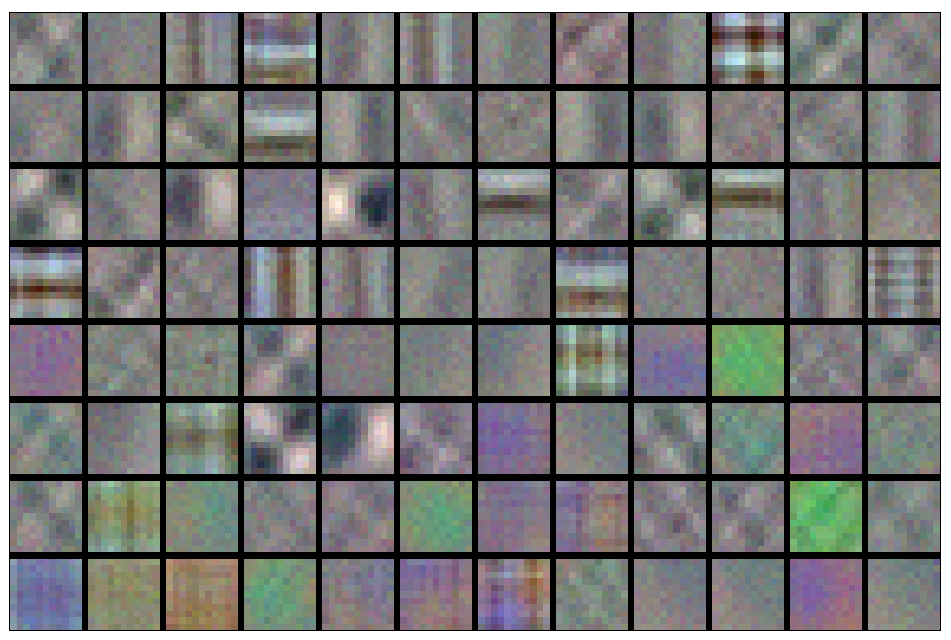
\includegraphics[scale=0.10]{images/l1_filters_iter5000.png}} \hspace{2mm}
\subfloat[15K Iterations]{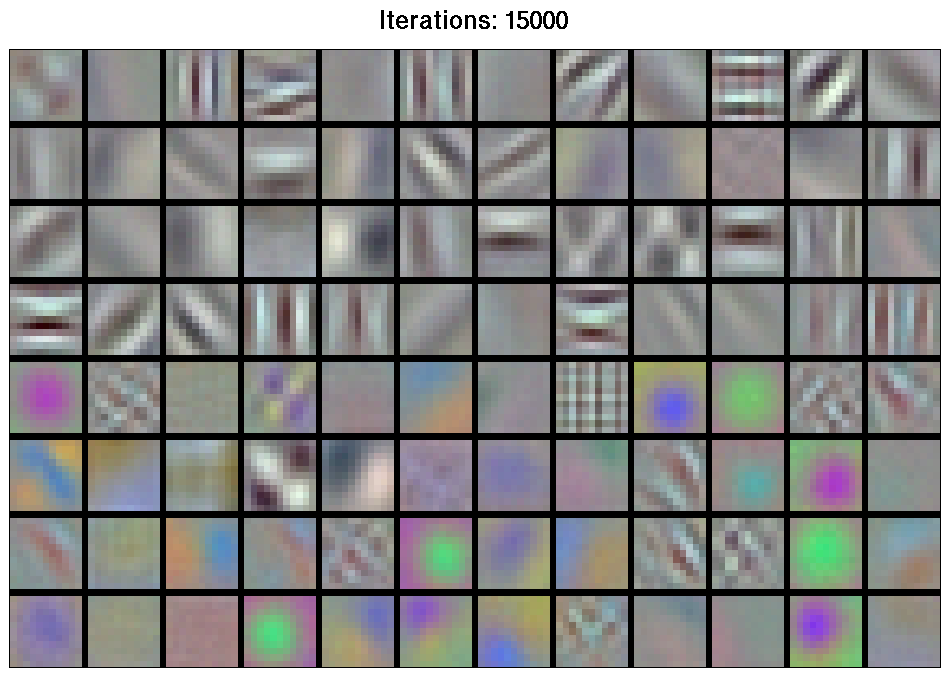
\includegraphics[scale=0.10]{images/l1_filters_iter15000.png}} \hspace{2mm}
\subfloat[305K Iterations]{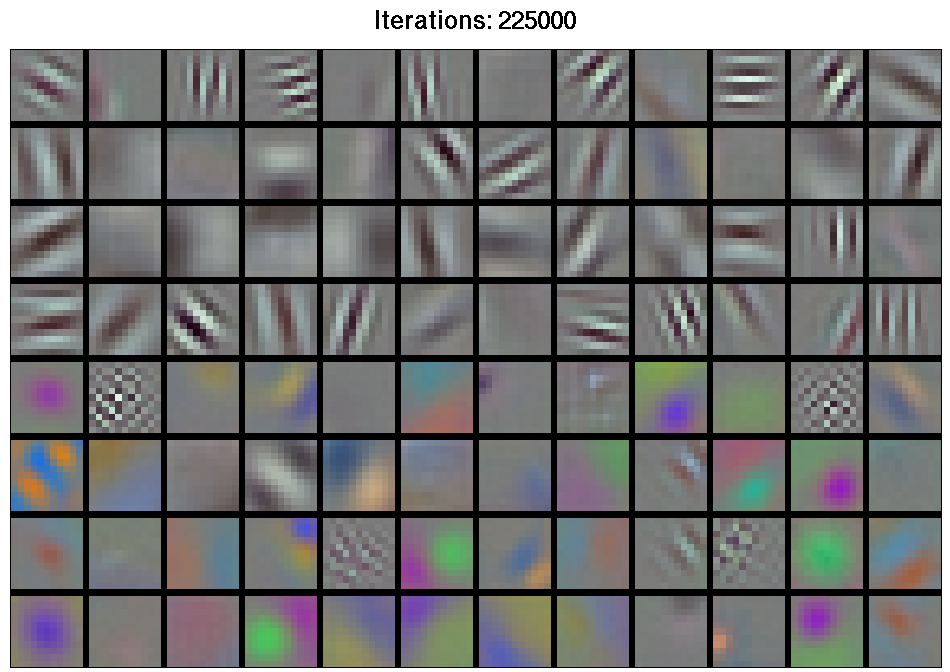
\includegraphics[scale=0.10]{images/l1_filters_iter225000.png}}
\caption{(a),(b),(c) show conv-1 filters after 5K, 15K and 305K iterations of training respectively. One pass (epoch) over the entire Imagenet-ILSVRC12 dataset takes approximately 5K iterations. Notice, that just after 15K iterations these filters closely resemble their final state.}
\begin{comment} Note: I have labeled 305K as 225K - I cannot get the same shape as of the 5K,15K for 305K. The filters look very similar and visually indistiguishable from 305K. If I have time later, I will make them all uniform.
\end{comment}
\label{fig:conv1}
\end{figure}


\setlength{\tabcolsep}{1pt}
\begin{table}[t!]
\begin{center}
\caption{Performance of 50-50 network for detection on pascal-voc-2007 challenge. (l5 is conv-5 and l7 is fc-7)}
\label{table:det-trajectory}
\scalebox{1.00}{
\begin{tabular}{|l|cccc|}
\hline
 & 50K & 105K & 205K & 305K \\
\hline
PASCAL-DET & 50.2 & 52.6 & 55.3 & 55.4 \\
SUN-CLS & 52.8 & 54.7 & 56.4 & 56.6 \\
\hline
\end{tabular}}
\end{center}
\end{table}
\setlength{\tabcolsep}{1.4pt}
The above analysis reinforces our belief that indeed majority of training required for generalization happens quite quickly as compared to the full training time of the network. This observation suggest that there may exist clever ways which can help us speed up the training.

